%%%%%%%%%%%%%%%%%%%%%%%%%%%%%%%%%%%%%%%%%%%%%%%%%%%%%%%%%%%%%%%%%%%%%%%%%%%%%%%%%%%%%%%%%%%%%%%%%%%%%
%
%   Version     : 2.0
%
%   Filename    : main.tex
%
%   Description : This is the main file for the LaTeX thesis proposal document template.
%                 The template is intended for use by BSCS students. 
%
%                It is assumed that you can learn how to use LaTeX on your own.
%                Please check/read the following online LaTeX book:
%
%                                 http://en.wikibooks.org/wiki/LaTeX
%     
%   Author      : Florante R. Salvador
%
%   Contributors: 1.  Karlo Campos 
%                     a. margin settings for DLSU thesis paper 
%   
%   Notes       : Please email florante.salvador@dlsu.edu.ph for comments, suggestions, ideas etc.
%
%   Reference:
%
%
%   History/Updates:
%      March 12, 2009 -- created version 1.0 for release to CSC701M (Methods of Research) students
%      May 30, 2009   -- updated Title page and Abstract for undergrad ST students
%
%      Feb 27, 2015 -- Created Version 2 (major overhaul): changed class to report, created a figures folder, 
%                               removed unnecessary packages, added new comments  based on Ethel Ong's slides
%
%%%%%%%%%%%%%%%%%%%%%%%%%%%%%%%%%%%%%%%%%%%%%%%%%%%%%%%%%%%%%%%%%%%%%%%%%%%%%%%%%%%%%%%%%%%%%%%%%%%%%%

%%%%%%%%%%%%%%%%%%%%%%%%%%%%%%%%%%%%%%%%%%%%%%%%%%%%%%%%%%%%%%%%%%%%%%%%%%%%%%%%%%%%%%%%%%%%%%%%%%%%%%%%%%%%%%%%%%%%%%%
%
%  Filename   : preamble.tex
%
%  Description: Preamble file to :
%               a. specify related packages
%               b. set margins, commands, etc.
%
%  Note       : Edit the margin settings for your own printer
%                  You may add your own commands, environments (it is assumed that you know what you're doing.)
%
%%%%%%%%%%%%%%%%%%%%%%%%%%%%%%%%%%%%%%%%%%%%%%%%%%%%%%%%%%%%%%%%%%%%%%%%%%%%%%%%%%%%%%%%%%%%%%%%%%%%%%%%%%%%%%%%%%%%%%%

%\documentclass[12pt,titlepage,onepage, letterpaper]{article}

\documentclass[12pt,titlepage,onepage, letterpaper]{report}


%
%-- specify related packages
%

%
% \usepackage[utf8x]{inputenc}
%

\usepackage{apacite}           %-- APA style citation 
                               %-- refer to http://www.ctan.org/tex-archive/biblio/bibtex/contrib/apacite/

%
%  \usepackage{ucs}
%


\usepackage{amsmath}           %-- American Math Society packages
\usepackage{amsfonts}
\usepackage{amssymb}


\usepackage{graphicx}          %-- graphicx package needed for including figures in JPG or PNG format
 
%
%\usepackage{graphics}          %-- graphics related package (this was commented out) use when image is in EPS format
%

\usepackage{verbatim}          %-- this package allows you to have multiple lines of comments by
                               %-- example:
                               %   \begin{comment}
                               %        ...your text here...
                               %   \end{comment}  

\usepackage{color}             %-- allows use of color with text
                               %-- example:  \textcolor{red}{This is the colored text in red.}

\usepackage{url}  %-- allows use of URLs example: \url{https:\ccs1.dlsu.edu.ph}


%
%-- set margins,  you may need to edit this for your own printer
%
\topmargin 0.0in
\oddsidemargin 0.0in
\evensidemargin 0.0in

\voffset 0.0in
\hoffset 0.5625in

\textwidth 5.75in
\textheight 8.5in


\parskip 1em
\parindent 0.25in

\bibliographystyle{apacite}            %-- use APA citation scheme

\hyphenation{ana-lysis know-ledge}     %-- LaTeX may not hyphenate correctly some words you use in your document
                                       %-- use \hyphenation to instruct LaTeX how to do it correctly, example above

\newcommand{\degree}{^{\circ}}         %-- use \newcommand to create your own "commands"
                                       %-- \newcommand works like the #define you learned in your COMPRO1 class

\newcommand{\etal}{et al.}


%\newcommand{\sinag}{\emph{Sinag}}
%\newcommand{\sinagtwo}{\emph{Sinag2}}

\newcommand{\figref}[1]{Figure \ref{#1}}
\newcommand{\appref}[1]{Appendix \ref{#1}}

%-- \newcommand{\Section}[1]{\section{#1}\setcounter{figure}{0}\setcounter{table}{0}}

%\newcommand{\shade}{\multicolumn{1}{|>{\columncolor[gray]{0.25}}c|}{}}
%\newcommand{\tableheader}[1]{\rowcolor{black}\color{white}{#1}}
%\newcommand{\cell}[2]{\multicolumn{1}{#1}{#2}}
%\newcommand{\definition}[2]{\textbf{\textit{#1}} --- #2}
%\newcommand{\itembit}[1]{\item \textbf{\textit{#1}}}
%\newcommand{\sgdef}[2]{\parbox[t][][t]{1.75in}{\textbf{#1}} \> \parbox[t][][t]{4.0in}{#2}\\\\}

%\newenvironment{sinagglossary}{\begin{flushleft}
%\begin{tabbing}
%\hspace{1.75in}\=\\}{\end{tabbing}\end{flushleft}}

\newcommand{\thestitle}[1]{{\Large \textsc{#1}}}


%---
%  \renewcommand{\thefigure}{\thesection.\arabic{figure}}
%  \renewcommand{\thetable}{\thesection.\arabic{table}}
%  \renewcommand{\contentsname}{Table of Contents}




                %-- includes LaTeX source file for the preamble 
                                  %-- include packages, sets the margin sequence, and many more... 
                                  %-- your job: check if the settings are suitable for your own printer

\graphicspath{{figures/}}  %-- figures is the name of the folder containing images JPG or PN

\begin{document}

%%%%%%%%%%%%%%%%%%%%%%%%%%%%%%%%%%%%%%%%%%%%%%%%%%%%%%%%%%%%%%%%%%%%%%%%%%%%%%%%%%%%%%%%%%%%%%%%%%%%%%
%
%   Filename    : title_page.tex 
%
%   Description : This file will contain your Title Page.
%                 
%%%%%%%%%%%%%%%%%%%%%%%%%%%%%%%%%%%%%%%%%%%%%%%%%%%%%%%%%%%%%%%%%%%%%%%%%%%%%%%%%%%%%%%%%%%%%%%%%%%%%%

\begin{titlepage}
\centering


%-- **EDIT** the following line to indicate your thesis title
\thestitle{Automatic Document Segmentation of Mobile Captured Medical Examination Forms in a Tele-Diagnosis System}

\vspace{1.75cm}
A Thesis Proposal\\
Presented to\\
the Faculty of the College of Computer Studies\\
De La Salle University Manila

\vspace{1.75cm}
In Partial Fulfillment\\
of the Requirements for the Degree of\\
Bachelor of  Science in Computer Science

\vspace{1.75cm}
by\\
%-- **EDIT** the following line to indicate your name 
\vspace{1cm}

SIBAYAN, Hannah Elien L. \\
VIRTUSIO, John Jethro C.  \\

\vspace{1.75cm}
%-- **EDIT** the following line to indicate your adviser's name 
Emerico AGUILAR \\
Adviser

\vspace{1.75cm}
\today
\end{titlepage}
              %-- includes LaTeX source file for the Title Page 
                                  %-- your job: **EDIT THIS FILE ** to indicate your own title, name, and thesis adviser's name


%%%%%%%%%%%%%%%%%%%%%%%%%%%%%%%%%%%%%%%%%%%%%%%%%%%%%%%%%%%%%%%%%%%%%%%%%%%%%%%%%%%%%%%%%%%%%%%%%%%%%%
%
%   Filename    : abstract.tex 
%
%   Description : This file will contain your abstract.
%                 
%%%%%%%%%%%%%%%%%%%%%%%%%%%%%%%%%%%%%%%%%%%%%%%%%%%%%%%%%%%%%%%%%%%%%%%%%%%%%%%%%%%%%%%%%%%%%%%%%%%%%%

\begin{abstract}
GetBetter, a telemedicine system, utilizes medical forms as means to collect data from patients. This paper discusses a proposed implementation of a suitable segmentation algorithm that will be used to extract fields from a digital photograph of a medical form. Several segmentation methods will be compared to arrive at the best possible implementation. If necessary the medical form is to be modified to enhance the segmentation. The segmentation process includes an implementation of a database system to store the data, an Optical character recognition module to translate the digital images to string and an android tablet application to take the photos of medical forms and communicate with the server. 

%
%  Do not put citations or quotes in the abract.
%


\begin{flushleft}
\begin{tabular}{lp{4.25in}}
\hspace{-0.5em}\textbf{Keywords:}\hspace{0.25em} & telemedecine, segmentation, optical character recognition \\
\end{tabular}
\end{flushleft}
\end{abstract}
                %-- this is the Abstract page
                                  %-- your job: **EDIT THIS FILE** to indicate your own abstract

\pagenumbering{roman}             %-- this will number pages as i, ii, iii, etc...
\setcounter{page}{2}

\tableofcontents                  %-- this command is used to generate the Table of Contents


\newpage
\listoffigures                    %-- this command is used to generate List of Figures

\newpage                       
\listoftables                     %-- this command is used to generate List of Tables

\newpage

\pagenumbering{arabic}            %-- this will number pages as 1, 2, 3, etc...
\setcounter{page}{1}              


%%%%%%%%%%%%%%%%%%%%%%%%%%%%%%%%%%%%%%%%%%%%%%%%%%%%%%%%%%%%%%%%%%%%%%%%%%%%%%%%%%%%%%%%%%%%%%%%%%%%%%
%
%   Filename    : chapter_1.tex 
%
%   Description : This file will contain your Research Description.
%                 
%%%%%%%%%%%%%%%%%%%%%%%%%%%%%%%%%%%%%%%%%%%%%%%%%%%%%%%%%%%%%%%%%%%%%%%%%%%%%%%%%%%%%%%%%%%%%%%%%%%%%%

\chapter{Research Description}
\label{sec:researchdesc}    %--note: labels help you with hyperlink editing (using your IDE)

\begin{comment}
Make sure to write a preamble for each chapter, i.e., a short description of what each chapter contains before 
the first section within the chapter.  The preamble can be written in about two to three sentences.
\end{comment}

\section{Overview of the Current State of Technology}
\label{sec:overview}

%
%   NOTE: You have to delete/replace the unnecessary paragraphs with your own text.
%

Telediagnosis is a diagnosis that occurs at a remote location and is based on the evaluation of data transmitted from devices that monitor the patient \cite{telediagnosis}. Computer systems connecting patients, midwives and doctors assist the telediagnosis process. For maximized collaboration and effectiveness, a good system design must adjust to the current business process the doctors and midwives are familiar with and not the other way around. The system must be a convenient tool for the people using it. Since the doctors and midwives are adapted to traditional ways such as writing on paper or vocal narration, it is best if they are not forced to divert from what they are already used to doing.

Replicating the current business process opens numerous computing challenges. One of which involves the management of paper forms. In the medical world, paper forms are used to contain and organize patient data in a uniform way. It is vital to the whole diagnosis process because it contains relevant information regarding the ailment of the patient and mismanagement of such forms can cause misdiagnosis and may endanger the patient’s life.  This study will propose a method to manage such forms in a digital space. It will present ideas relevant to the problem, such as image segmentation, storage, retrieval, structuring and digitalization of paper forms. The study will also describe the process of deciding which method is best for the segmentation of digital paper forms.

A digital image of a medical form is a good medium for storing data because it guarantees that the medical form will be stored as it is but it is not a good medium for analysis.  Data stored as an image occupies a huge amount of space and in limited bandwidth transferring images is significantly slower and may even be impossible. In scale, the whole system may fail because of it’s inability to transfer huge amounts of data.  This study will provide an approach how to get the useful data from digital images of paper forms and to minimize the storage space used. 

\begin{comment}
\figref{fig:disneystock} shows a graph of the performance of Disney stock from the 1980s to 2012.
  
%--- the following example shows how to include a figure in PNG format
\begin{comment}[t]                %-- use [t] to place figure at top, [b] to place at the bottom, [h] for here
   \centering                    %-- use this to center the figure
   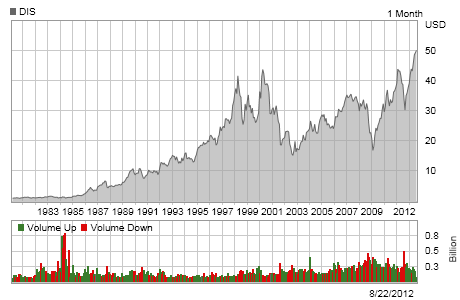
\includegraphics{DisneyChart.png}      %-- include image file named as "disneychart.png" 
   \caption{This is the figure's caption -- Disney stock chart}
    \label{fig:disneystock}
\end{comment}


\begin{comment}
 \item \citeA{kartch:2000:ERA} compared reaction times...
 \item In a recent study of reaction times \cite{kartch:2000:ERA}...
 \item In \citeyearNP{kartch:2000:ERA}, \citeauthor{kartch:2000:ERA} compared reaction times...
 \item \shortciteA{fedkiw:2001:VSO} compared reaction times... 
 \item In a recent study of reaction times \cite{fedkiw:2001:VSO}...
 \item In \citeyearNP{fedkiw:2001:VSO}, \shortciteauthor{fedkiw:2001:VSO}, compared reaction times...
\end{comment}



\section{Research Objectives}
\label{sec:researchobjectives}

\subsection{General Objective}
\label{sec:generalobjective}

To create a system that stores and retrieves useful information from digital images of paper forms to provide a fast and convenient way for viewing the information on a screen.   


\subsection{Specific Objectives}
\label{sec:specificobjectives}

%
%  \begin{comment} ... \end{comment} is used for multiple lines of comment
%



\begin{comment}

This subsection is an elaboration of the general objective.  It states the specific steps that must be undertaken to accomplish the
general objective.  These objectives must be specific, measurable, attainable, realistic, time-bounded.  Each specific objective may
start with ``to design/survey/review/analyze''

Studying a particular programming language or development tool (e.g., to study Windows/Object-Oriented/Graphics/C++ programming) to 
accomplish the general objective is inherent in all thesis and, therefore, must not be included here.


%
% IPR acknowledgement: the following sentences and examples are from Ethel Ong's slides 
%     on Research Objectives
%

How to formulate your research objectives:
1. Identify what research steps do you need to perform to achieve your general objective.
2. Identify the questions that must be answered for you to achieve your general objective.
    Thereafter, convert these questions into action statements


Example #1:

Research Question:
  What are the general features of a web-based learning environment?

Specific Objective:
   To review existing web-based learning environment that teaches language learning for children


Example #2:

Research Question:
   How will you represent commonsense knowledge for use by computer systems?

Specific Objective:
   To identify knowledge representation approaches used by existing story generation systems

Example #3:
Research Question:
   What types of storytelling knowledge are needed to generate stories?

Specific Objective:
    To identify the different types of storytelling knowledge used in generating stories

Example #4:
Research Question:
    What machine learning approaches will you utilize?

Specific Objective:
    To determine existing machine learning algorithms [that can be used in training the computer system to detect cyberbullying cases] 

Example #5: Research Question:
    How will your research output be evaluated?

Specific Objective:
    To define evaluation metrics for validating the accuracy of the translation

\end{comment}

%
%  The following are example specific objectives; replace them with your own 
%

\begin{enumerate}
   
   \item To provide a modified version of the current medical examination form that will be more appropriate in the process.
   \item To implement an algorithm that extracts the medical examination form from the mobile captured image.
   \item To prepare the extracted image for segmentation by implementing a dewarping algorithm.
   \item To implement an algorithm that extracts and identifies the multiple sections of the form.
   \item To extract the data on the identified sections as strings.
   \item To create a database that stores extracted strings of the form.
   
\end{enumerate}


\section{Scope and Limitations of the Research}
\label{sec:scopelimitations}

The study focuses on the segmentation of specific types of forms and its implementation will cover selected image processing algorithms from reviewed studies. Currently, medical examination forms exists for the use of the GetBetter system. These forms are to be modified to be more compatible with the algorithms to be used. The test images that will be used in the study will mainly be a variety of mobile captured images of the modified forms.

The performance of image segmentation techniques depend heavily on the quality of the image. It is important to note that the quality of the image may vary depending on the hardware used to take the picture, on the physical condition of the paper form and on the circumstances the image was taken. Because of this variance, it cannot be guaranteed that image segmentation process will work for all kinds of images and conditions, however an algorithm that will work under the worst condition will be employed to guarantee maximum effort and performance instead. For the purpose of GetBetter, the test images in this study will be those which are captured on a Samsung tablet since that is what is currently being used.


\begin{comment}

%
% IPR acknowledgement: the sentences inside this comment are from Ethel Ong's slides on Scope and Limitations of the Research
%
Generally, one paragraph should be allotted for each of your research objectives.

Each paragraph contains a brief overview of the concept/theory and the purpose of doing the associated objective.

Each paragraph also includes a description of the scope/limitation of your study.

* Please refer to the slides for examples.

\end{comment}


\section{Significance of the Research}
\label{sec:significance}

People are growing to be more dependent on technology and because of this almost everything is becoming digital including physical documents. Providing a way to make these documents presentable and accessible on various devices is now an important matter.

The GetBetter Tele-Diagnosis System lacks the functions which can support the transformation of the forms in images into a better digital representation of the form. Currently the system does not provide an interface that allows doctors to obtain sections of a patient’s medical examination form separately. Providing functions that will allow a systematic approach in the diagnosis process is a step further in enabling the doctors to become more productive and the system more convenient.

The resulting database of images which contain information about the patients can then be used by an Optical Character Recognition system to replace the images with actual values represented as strings or numbers. This will produce a more comprehensible information that the users and system can utilize.

%
% IPR acknowledgement: the following list of items are from Ethel Ong's slides on Significance of the Research
%
\begin{comment}
\begin{itemize}
\item  What is the relevance of your work to the computer science community? 

\begin{itemize} 
\item What will be your technical contributions, in terms of algorithms, or approaches, or new domain? 
\item What is your value-added compared to existing systems? 
\end{itemize}

\item What will be your contributions to society in general? 
    \begin{itemize}
      \item Who will benefit from your system? 
      \item Who are your target users and how will this system benefit them? 
   \end{itemize}
\end{itemize}

If applicable, describe possible commercialization and/or innovation in your research.
\end{comment}


               %-- includes LaTeX source file for Chapter 1: Research Description
                                  %-- your job: **EDIT THIS FILE** to indicate your own research description

%%%%%%%%%%%%%%%%%%%%%%%%%%%%%%%%%%%%%%%%%%%%%%%%%%%%%%%%%%%%%%%%%%%%%%%%%%%%%%%%%%%%%%%%%%%%%%%%%%%%%%
%
%   Filename    : chapter_2.tex 
%
%   Description : This file will contain your Review of Related Literature.
%                 
%%%%%%%%%%%%%%%%%%%%%%%%%%%%%%%%%%%%%%%%%%%%%%%%%%%%%%%%%%%%%%%%%%%%%%%%%%%%%%%%%%%%%%%%%%%%%%%%%%%%%%

\chapter{Review of Related Literature}
\label{sec:relatedlit}

\section{Studies on Object Detection for Paper Forms}

A study done by \citeA{george13}, uses Canny Edge Detection to find objects in the image. To identify the object in the image, a query image is used as a template to be a point of comparison. Correlation coefficient with the edges of template image for each object found in the image is computed and whichever object has the highest correlation value must be the object of interest. Though the study has merits it also comes with problems such as, the size of the template image and search image will never be the same and that will significantly affect the correlation coefficient.  Thus a technique that is independent from the image size must be explored. 


One possible technique dependent from the size of the image is shape analysis.  A paper done by \citeA{teh89} discusses a technique used to identify  the dominant points in an enclosed curvature using the assumptions that dominant points are located at maximum curvatures of the shape. Thus a square or rectangle contains four dominant points, Octagon with eight and so on.  One possible problem with this technique is differentiating noise shapes with important shapes. The location of important shapes must be clearly defined so that out of placed shapes will be discarded.  This technique can be very useful on detecting the fields on the form, however, similar to the object detection by the canny algorithm,  this technique does not take advantage of colors.


If the form has distinct colors, color based image segmentation techniques can be used.\shortciteA{rathore12} proposes the use of  L*A*B as features and K- means to segment the image. This technique can be applied to the paper forms by assigning distinct colors to objects of interests in the image.  By knowing the distinct colors, it can easily be found in the image by K-means.  


Correlation coefficient, Shape analysis, and color based segmentation are useful techniques if the location of the object is not known. However for paper forms, each location of the field is already known, given that the type of paper form can be identified. It is the paper form itself that has an unknown location within the image. \shortciteA{nguyen11} discusses an approach used on an multiple choice answer sheet that takes advantage of the known location. They transform the paper in the correct orientation using hough transform and normalize it through resizing. By doing so, each objects in the multiple choice answer sheet can be extracted using its known normalized location and size.



\begin{table}[h]
	\begin{center}
		\begin{tabular}{| l | l |} 
			\hline
			Author & Techniques Used For Object Detection \\ [0.5ex] 
			\hline\hline
			\citeA{george13} & Canny Edge Detection algorithm, Correlation  \\  [0.5ex]
			\hline
			\shortciteA{teh89} & Curvature Measure, Number of points\\ [0.5ex]
			\hline
			\shortciteA{rathore12} & L*A*B features, K-means\\ [0.5ex]
			\hline
			\shortciteA{nguyen11} &Hough Transform, Normalization\\ [0.5ex] 
			\hline
		\end{tabular}
		\caption{Object Detection Summary}
		\label{table:1}
	\end{center}
\end{table}



\section{Studies on Improving Readability}


Once the form has been found in the image, to improve readability it must be dewarped to fix the skewness and orientation. A paper by  \shortciteA{stam08} proposes a two step dewarping process. The first step is to map the projection of a warped image to a 2D rectangular box . Next step is fine adjustment of the letters by looking for the words and aligning it. Though for the purpose of the forms the fine adjustment step won’t work because the proposed word detection does not work on handwritten characters.  Projecting the form to a 2D rectangular box will make it easier find the fields because it can then be mapped using its location on the x y plane. 


After transformation, to aid the field searching and readability the document should be cleaned of its noise. Depending on the type of noise \shortciteA{farahmand13} proposes different kinds of technique like thresholding, fuzzy logic based, and morphology based.  It is important to identify the type of noise the forms will be most likely be exposed to before implementing such algorithms. 

\begin{table}[h]
	\begin{center}
		\begin{tabular}{| l | l |} 
			\hline
			Author & Techniques Used for improving readability \\ [0.5ex] 
			\hline\hline
			\shortciteA{stam08} & Projection of curved image to 2D rectangular box \\ [0.5ex]
			\hline
			\shortciteA{farahmand13} & Noise Reduction \\ [0.5ex]
			\hline
		\end{tabular}
		\caption{Improving Readability Summary}
		\label{table:1}
	\end{center}
\end{table}



\section{Image Segmentation}


\shortciteA{huang15} presented a method of workpiece recognition and location based on Open Source Computer Vision (OpenCV). The paper mentions how workpiece recognition and location technology is important in automatic production. The method has three stages which are preprocessing, contour extraction, and workpiece recognition and location. The preprocessing includes image graying, mean filter, adaptive threshold segmentation, and image binarization. Contour extraction makes use of the findContours function of OpenCV on the resulting binary image of the preprocessing stage. The contours with small perimeters or complex shapes are removed and the remaining contours are filled up and used for another contour extraction with the findContours function. A template image, which is the image of the workpiece, undergoes the same process to be used for template matching in the next stage. Using the OpenCV function matchShapes, the contours of the first image, or the identifying image, is matched with the contours of the template. Once the shapes match, the position is obtained by calculating the mass center of its contour. Based on experimental results, the method can realize workpiece recognition and location and can satisfy real time demand.


In a study by \shortciteA{gupta06}, document layouts are extracted automatically and segments of the document are analyzed and bounded given its spatial arrangement. The process involves two major steps which are layout extraction and layout analysis. Layout extraction deals with merging rectangular regions until a global layout structure is generated. Layout analysis involves defining a model of a paper layout, performing feature extraction on the resulting image, and then classification. Technical documents such as scanned journals and conference proceedings were used for testing. The system was implemented using Visual C++ and Open Source Computer Vision (OpenCV) library.


\shortciteA{patel15} presented a low cost optical mark recognition (OMR) system called CheckIt. The system is developed using Python and the Open Source Computer Vision (OpenCV) library for the back end and Android for the front end. It is low cost because it utilizes open source technology and does not need a scanning hardware. The method involves image graying, resizing, adaptive histogram equalization, adaptive thresholding, blurring, canny edge detection, contour extraction, affine transformation, and score calculation. Based on the study’s results, the algorithm has high accuracy and speed. It was tested on 310 images with an average processing time of 3 seconds per image.

\begin{table}[h]
	\begin{center}
		\begin{tabular}{| l | l |} 
			\hline
			Authors & Techniques Used for Image Segmentation \\ [0.5ex]
			\hline\hline
			\shortciteA{huang15} & Contour Extraction and Template Matching using the OpenCV library\\ [0.5ex]
			\hline
			\shortciteA{gupta06} &
			Segmentation algorithms using the OpenCV library \\ [0.5ex]
			\hline
			\shortciteA{patel15} &
			Contour Extraction using the OpenCV library\\ [0.5ex]
			\hline
		\end{tabular}
		\caption{Image Segmentation Summary}
		\label{table}
	\end{center}
\end{table}

\section{Optical Character Recognition}


\shortciteA{vuong14} presented a multilanguage name card reader on an Android platform. The method was implemented with the Open Source Computer Vision (OpenCV) library and Tesseract Optical Character Recognition (Tesseract OCR). The proposed system has six steps which are language selection, retrieval of image from the camera or SD card, preprocessing, optical character recognition (OCR), pattern matching, and contact information adding. Preprocessing involves image resizing, noise reduction, card area detection, image graying, and locally adaptive binarization. The Tesseract OCR is then used on the resulting binary image. Different information is extracted from the OCR step and to deal with this the content is matched with a predefined format to only obtain the necessary contents. The final step then adds the information extracted to the contact list of the device. Although the system is unable to correctly extract information in cases with complex background and blurred image, the results still showed a satisfactory number with high accuracy over 90%.


\begin{table}[h]
	\begin{center}
		\begin{tabular}{| l | l |} 
			\hline
			Authors &
			Techniques Used for Optical Character Recognition \\ [0.5ex] 
			\hline\hline
			\shortciteA{vuong14} &  \parbox[t]{3in}{Segmentation algorithms \par using the OpenCV
				library and Tesseract Optical Character Recognition} \\ [0.5ex]
			\hline
		\end{tabular}
		\caption{Optical Character Recognition Summary}
		\label{table}
	\end{center}
\end{table}







\begin{comment}
%
% IPR acknowledgement: the contents withis this comment are from Ethel Ong's slides on RRL.
%
Guide on Writing your RRL chapter

1. Identify the keywords with respect to your research
One keyword = One document section
Examples: 2.1 Story Generation Systems
2.2 Knowledge Representation

2.  Find references using these keywords

3.  For each of the references that you find,
Check: Is it relevant to your research?
Use their references to find more relevant works.

4. Identify a set of criteria for comparison.
It will serve as a guide to help you focus on what to look for

5. Write a summary focusing on -
What: A short description of the work
How: A summary of the approach it utilized
Findings: If applicable, provide the results
Why: Relevance to your work

6. At the end of each section,  show a Table of Comparison of the related works 
and your proposed project/system

\end{comment}

\begin{comment}
\section{Review of Related Paper}
This section contains a review of research papers that:
%
% IPR acknowledgement: the following list of items are from Ethel Ong's slides RRL.
%
\begin{itemize}
\item Describes work on a research area that is similar or relevant to yours
\item Describes work on a domain that is similar or relevant to yours
\item Uses an algorithm that may be useful to your work
\item Uses a software / tool that may be useful to your work
\end{itemize}

\section{Review of Related Software}
This section contains a review of software systems that:
%
% IPR acknowledgement: the following list of items are from Ethel Ong's slides on RRL.
%
\begin{itemize}
\item Belongs to a research area similar to yours
\item Addresses a need or domain similar to yours
\item Is your predecessor
\end{itemize}

\end{comment}














               %-- includes LaTeX source file for Chapter 2: Review of Related Literature
                                  %-- your job: **EDIT THIS FILE** to indicate your review of related literature 

%%%%%%%%%%%%%%%%%%%%%%%%%%%%%%%%%%%%%%%%%%%%%%%%%%%%%%%%%%%%%%%%%%%%%%%%%%%%%%%%%%%%%%%%%%%%%%%%%%%%%%
%
%   Filename    : chapter_3.tex 
%
%   Description : This file will contain your Research Methodology.
%                 
%%%%%%%%%%%%%%%%%%%%%%%%%%%%%%%%%%%%%%%%%%%%%%%%%%%%%%%%%%%%%%%%%%%%%%%%%%%%%%%%%%%%%%%%%%%%%%%%%%%%%%

\chapter{Research Methodology}
This chapter lists and discusses the specific steps and activities that will be performed by the proponent to accomplish the project. 
The discussion covers the activities from pre-proposal to Final Thesis Writing.  It also includes an initial discussion on the theoretical
framework to be followed.

\section{Research Activities}

\subsection*{3.1.1 Testing different image segmentation approaches.}


Each member of the group will try a different, approach for image segmentation. The results will be compared and the best approach will be used as the primary algorithm for image segmentation. This is done to ensure that the best possible algorithm is implemented, and the system will work as best as possible.

\subsection*{3.1.2 Redesigning of medical forms}

Depending on the image segmentation technique, the medical form may be redesigned to aide the process. The member testing the image segmentation technique may opt to redesign the form if necessary. 

\section{Calendar of Activities}

\begin{figure}[h]                %-- use [t] to place figure at top, [b] to place at the bottom, [h] for here
	\centering                    %-- use this to center the figure
	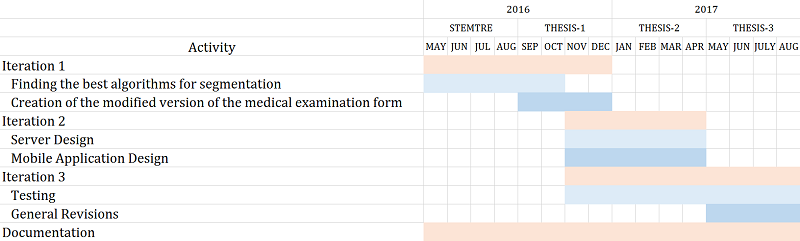
\includegraphics{gant.png}      %-- include image file named as "disneychart.png" 
	\caption{Gantt Chart of Activities}
	\label{fig:disneystock}
\end{figure}





               %-- includes LaTeX source file for Chapter 3: Research Methodology
                                  %-- your job: **EDIT THIS FILE** to indicate your research methodology

\appendix                         %-- used to specify appendices
%%%%%%%%%%%%%%%%%%%%%%%%%%%%%%%%%%%%%%%%%%%%%%%%%%%%%%%%%%%%%%%%%%%%%%%%%%%%%%%%%%%%%%%%%%%%%%%%%%%%%%
%
%   Filename    : appendix_A.tex 
%
%   Description : This file is one of the appendices. 
%                 
%%%%%%%%%%%%%%%%%%%%%%%%%%%%%%%%%%%%%%%%%%%%%%%%%%%%%%%%%%%%%%%%%%%%%%%%%%%%%%%%%%%%%%%%%%%%%%%%%%%%%%

\chapter{Diagrams and Other Documentation Tools}
\label{sec:appendixa}

\section{Process Flow}

\subsection*{The system has two parts: client and server.}


\subsection{Client Side}

The client is implemented on an android tablet. The client is responsible for taking pictures, segmenting it to relevant parts and extracting the relevant information as strings. OpenCV will be used as the primary library for image operations and Tesseract as the primary library for Optical character recognition.


\begin{figure}[h]                %-- use [t] to place figure at top, [b] to place at the bottom, [h] for here
	%-- use this to center the figure
	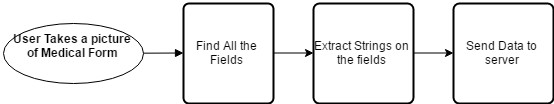
\includegraphics{client.png}      %-- include image file named as "disneychart.png" 
	\caption{Client Side}
	\label{fig:disneystock}
\end{figure}

\pagebreak
\subsection{Server Side} 

The server side is responsible for storing the data received from the client. MySQL will be used as the database and the server side will be implemented on java. 

\begin{figure}[h]                %-- use [t] to place figure at top, [b] to place at the bottom, [h] for here
	\centering                    %-- use this to center the figure
	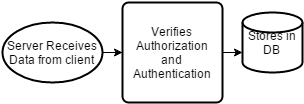
\includegraphics{server.png}      %-- include image file named as "disneychart.png" 
	\caption{Server Side}
	\label{fig:disneystock}
\end{figure}

\pagebreak

\section{Medical Examination Forms currently used by the GetBetter Tele-Diagnosis System.}

\subsection{First Form} 
\begin{figure}[h]                %-- use [t] to place figure at top, [b] to place at the bottom, [h] for here
	\centering                    %-- use this to center the figure
	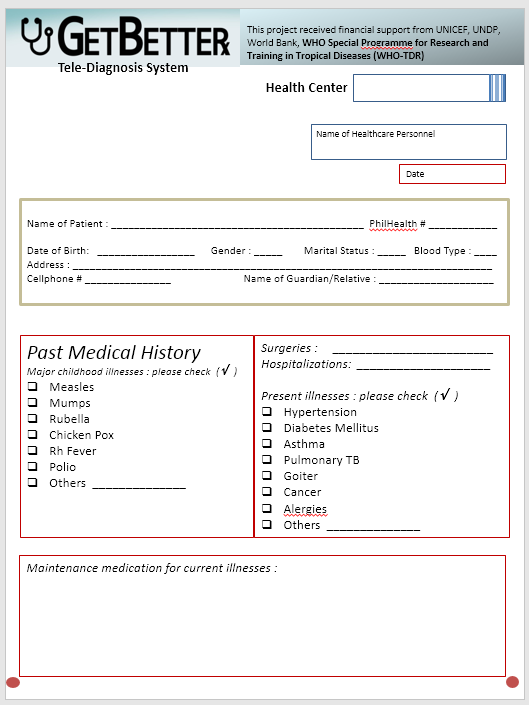
\includegraphics{form1.png}      %-- include image file named as "disneychart.png" 
	\label{}
\end{figure}

\pagebreak
\subsection{Second Form}
\begin{figure}[h]                %-- use [t] to place figure at top, [b] to place at the bottom, [h] for here
	\centering                    %-- use this to center the figure
	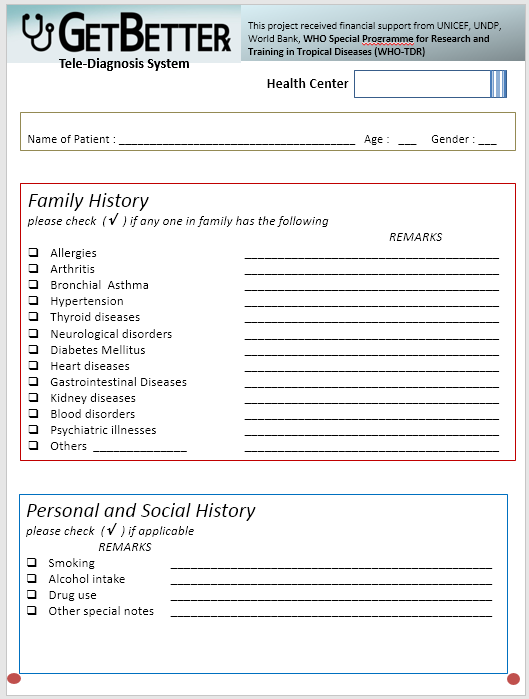
\includegraphics{form2.png}      %-- include image file named as "disneychart.png" 
	\label{}
\end{figure}

\pagebreak
\subsection{Third Form}
\begin{figure}[h]                %-- use [t] to place figure at top, [b] to place at the bottom, [h] for here
	\centering                    %-- use this to center the figure
	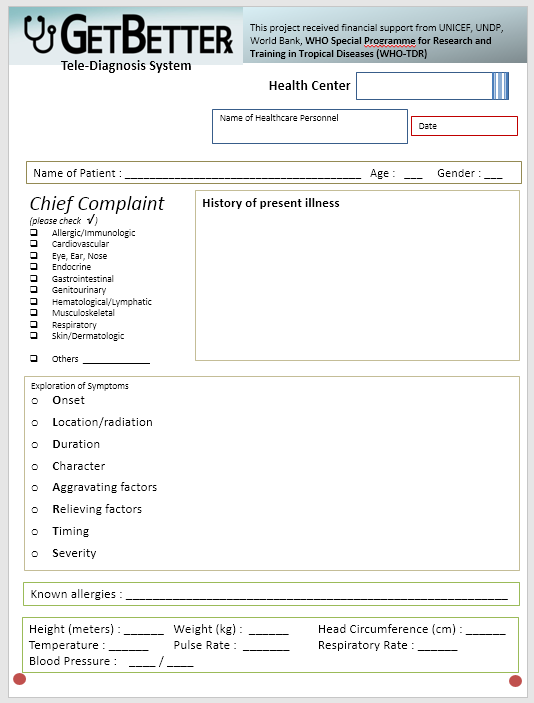
\includegraphics{form3.png}      %-- include image file named as "disneychart.png" 	
	\label{}
\end{figure}


\pagebreak

\section{Medical Examination Forms in preparation for the Optical Character Recognition system}

\subsection{First Form} 
\begin{figure}[h]                %-- use [t] to place figure at top, [b] to place at the bottom, [h] for here
	\centering                    %-- use this to center the figure
	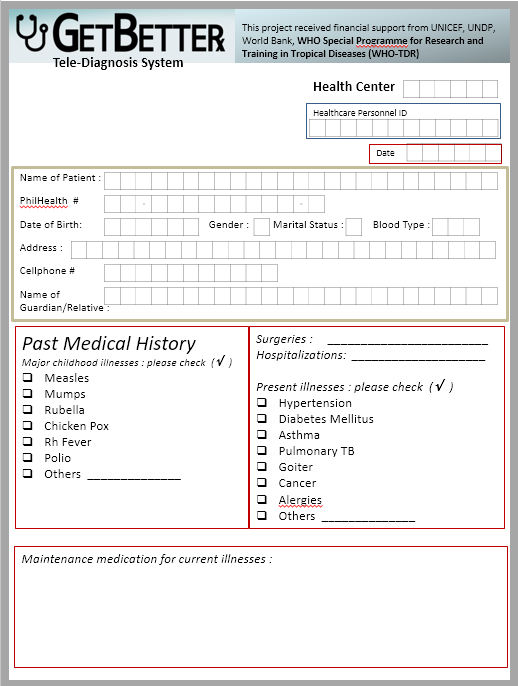
\includegraphics{_newform1.png}      %-- include image file named as "disneychart.png" 
	\label{}
\end{figure}

\pagebreak
\subsection{Second Form}
\begin{figure}[h]                %-- use [t] to place figure at top, [b] to place at the bottom, [h] for here
	\centering                    %-- use this to center the figure
	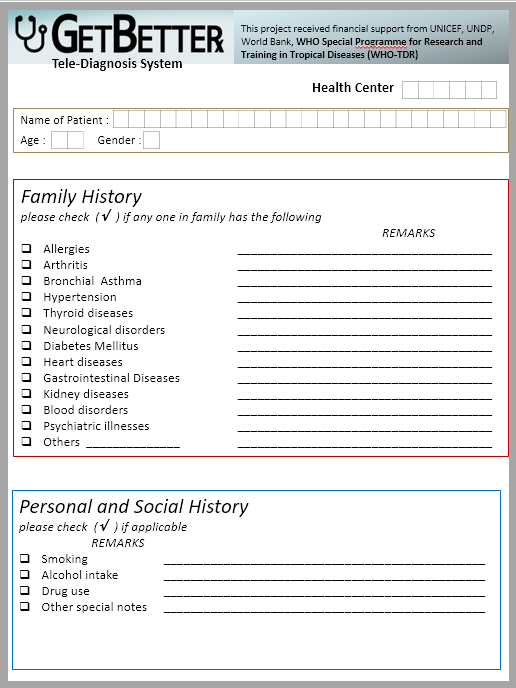
\includegraphics{_newform2.png}      %-- include image file named as "disneychart.png" 
	\label{}
\end{figure}

\pagebreak
\subsection{Third Form}
\begin{figure}[h]                %-- use [t] to place figure at top, [b] to place at the bottom, [h] for here
	\centering                    %-- use this to center the figure
	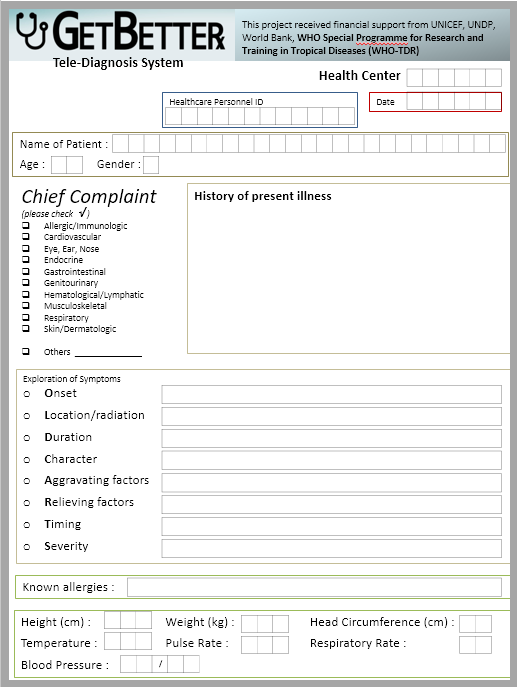
\includegraphics{_newform3.png}      %-- include image file named as "disneychart.png" 	
	\label{}
\end{figure}

\pagebreak
\subsection{Fourth Form}
\begin{figure}[h]                %-- use [t] to place figure at top, [b] to place at the bottom, [h] for here
	\centering                    %-- use this to center the figure
	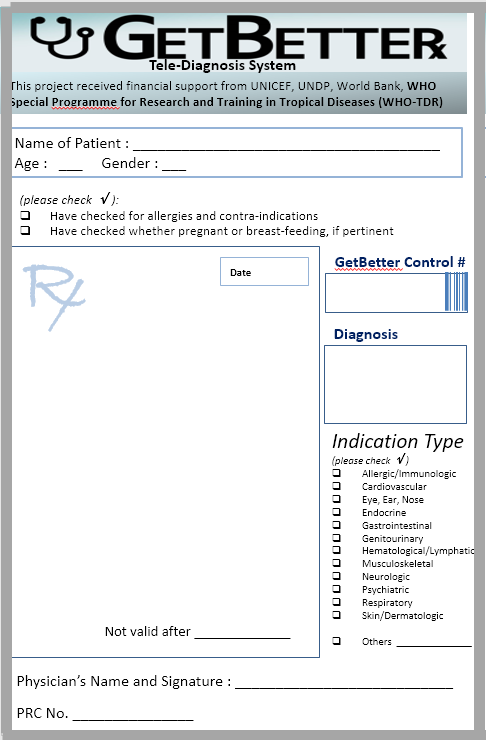
\includegraphics{_newform4.png}      %-- include image file named as "disneychart.png" 	
	\label{}
\end{figure}

\pagebreak
\subsection{Fifth Form}
\begin{figure}[h]                %-- use [t] to place figure at top, [b] to place at the bottom, [h] for here
	\centering                    %-- use this to center the figure
	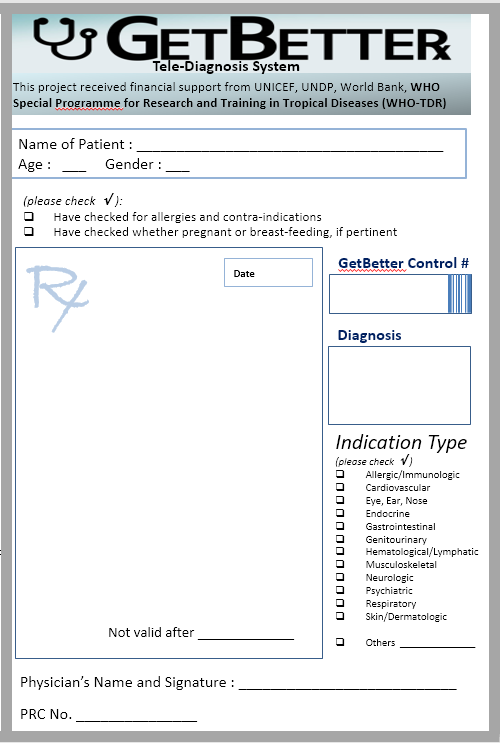
\includegraphics{_newform5.png}      %-- include image file named as "disneychart.png" 	
	\label{}
\end{figure}








              %-- includes LaTeX source file for Appendix A
                                                 %-- your job: **CREATE/EDIT** your own source file for the appendices
%%%%%%%%%%%%%%%%%%%%%%%%%%%%%%%%%%%%%%%%%%%%%%%%%%%%%%%%%%%%%%%%%%%%%%%%%%%%%%%%%%%%%%%%%%%%%%%%%%%%%%
%
%   Filename    : appendix_B.tex 
%
%   Description : This file will contain one of your appendices.
%                 
%%%%%%%%%%%%%%%%%%%%%%%%%%%%%%%%%%%%%%%%%%%%%%%%%%%%%%%%%%%%%%%%%%%%%%%%%%%%%%%%%%%%%%%%%%%%%%%%%%%%%%

\chapter{Theoretical and/or Conceptual Framework}
\label{sec:appendixb}

\section{Image Pre-Processing}
Image Pre-Processing involves the transformation of raw digital images of paper forms to a more useful digital image. This process removes noise and outputs a gray-scale and a binary version of the image to aide the image segmentation process. Farahmand, et al. (2013), proposed different approaches to clean image. These approaches is applicable on our images and will be the main reference for cleaning the images. 

\section{Image Segmentation}
Image segmentation is the process of extracting all relevant parts of the	image. The main goal is to extract and identify each field in the medical form. Different image segmentation techniques relevant to the study includes, color, contour and location based segmentation discussed by different authors in the related literature. Different approaches will be tried to determine the best and most robust way. 

\section{Optical Character Recognition}
Optical Character Recognition translates digital images of characters to string characters. This process is necessary because the data retrieved in the medical forms will be stored as strings. Tesseract, an open-source Optical Character Recognition (OCR) engine that has a very high correct recognition rate (Vuong and Do, 2014) will be used . Tesseract OCR works well in an Android Application as seen on Vuong and Do’s (2014) proposed system. Similarly to OpenCV, it only needs to be imported and its functions can easily be used.

%%%%%%%%%%%%%%%%%%%%%%%%%%%%%%%%%%%%%%%%%%%%%%%%%%%%%%%%%%%%%%%%%%%%%%%%%%%%%%%%%%%%%%%%%%%%%%%%%%%%%%
%
%   Filename    : appendix_C.tex
%
%   Description : This file will contain information about your Resource Persons
%                 
%%%%%%%%%%%%%%%%%%%%%%%%%%%%%%%%%%%%%%%%%%%%%%%%%%%%%%%%%%%%%%%%%%%%%%%%%%%%%%%%%%%%%%%%%%%%%%%%%%%%%%

\chapter{Resource Persons}
\label{sec:appendixc}

%
%  Indicate your resource persons here:
%
%	<full name and title, e.g., Dr. Juan de la Cruz>
%	<profession, e.g., faculty>
%	<department, e.g., College of Computer Studies>
%	<name of institution, e.g., De La Salle University>
%	<e-mail address>
%
%

%
%  the following shows 3 examples, replace entries with your own
%
\newcommand{\resperson}[4]{\textbf{#1} \\ #2 \\ #3 \\ \url{#4}\vspace{0.5em}\\}

\resperson{Emerico Aguilar}{Adviser}{College of Computer Studies\\De La Salle University-Manila}{emerico.aguilar@dlsu.edu.ph}


%\bibliographystyle{apacite}       %-- specified APA style for bibliograpy
                                  %-- more details about APA style citation can be found in www.ctan.org/tex-archive/biblio/bibtex/contrib/apacite/

                                  %-- bibliographic entries are handled via bibtex; refer to www.bibtex.org for more details


\bibliography{myreferences}       %-- the file "myreferences.bib" is a sample bibliography (bib) from SIGGRAPH 
                                  %-- your job: **CREATE/EDIT** your own bibliography file  

\end{document}

